\subsection{Parallelization of tridag}
It is worth looking into the given function \textbf{tridag} and why it is not
immediately parallelizable. Inside \textbf{tridag} we have a couple of
loops which each performs cross iteration dependencies.

\begin{figure}[!ht]
	\centering
		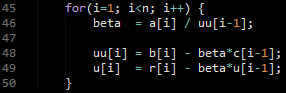
\includegraphics[scale=1]{input/figures/tridag_loop1.png}
		\caption{First loop of \textbf{tridag}.\label{fig:tridag_loop1}}
\end{figure}

In Figure \ref{fig:tridag_loop1} we can see how each iteration accesses
the result of \emph{u} from the previous iteration. Hence this is not
immedeatly parallelizable.

\begin{figure}[!ht]
	\centering
		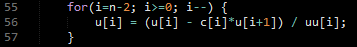
\includegraphics[scale=1]{input/figures/tridag_loop2.png}
		\caption{Second loop of \textbf{tridag}.\label{fig:tridag_loop2}}
\end{figure}

When looking at the other loop, shown in Figure \ref{fig:tridag_loop2}, we can see that each iteration access \emph{u} of the following iteration before it is overwritten by its respected iteration.
To be able to execute \textbf{tridag} in parallel these issues must be dealt with first.
